\documentclass[30pt,a4paper,landscape,headrule,footrule]{foils}
\usepackage{graphicx}
\usepackage{pslatex}
\usepackage{color}
\usepackage{listings}
\usepackage{times}
\usepackage[top=1.5cm, bottom=3.5cm, left=2cm, right=2cm]{geometry} 

\headsep 1.5cm

\lstset{%
	language=C,
	keywordstyle={\color{blue}},
	basicstyle=\scriptsize,
	stringstyle=\ttfamily
}

\title{RedirFS \\ Pimp your filesystem \\ [1cm]}
\author{\tt{Frantisek Hrbata} \\ \tt{frantisek.hrbata@redirfs.org} \\
\tt{www.redirfs.org} \\ [1cm]}
\date{October 30, 2007}

\leftheader{Redirecting FileSystem}
\rightheader{}
\MyLogo{LinuxAlt 2007}

\begin{document}
\maketitle

\foilhead[-2cm]{Content}
\rightheader{Content}
\begin{itemize}
\item Virtual Filesystem Switch
\item Stackable Filesystems
\item Linux Security Module
\item Dazuko
\item Redirecting FileSystem
\item Filters
\end{itemize}

%-------------------------------------------------
\foilhead[-2cm]{Virtual Filesystem Switch}
\rightheader{Virtual Filesystem Switch}

\begin{itemize}
\item one of first implementation in SunOS 2.0 by Sun Microsystems in 1985
\item handles system calls related to filesystems
\item provides common interface to several kinds of filesystems
\item abstraction layer between user space processes and filesystem drivers
\end{itemize}

%-------------------------------------------------
\foilhead[-2cm]{Virtual Filesystem Switch}
\begin{itemize}
\item common filesystem model able to handle different filesystem types
\item filesystem drivers have to translate their physical organization to the
VFS' common model
\item caches to eliminate calls to filesystem drivers
\end{itemize}

%-------------------------------------------------
\foilhead[-2cm]{Filesystems Classes}

\begin{itemize}
\item Disk-based filesystems -- ext*, reiserfs, ufs, iso9669, hpfs
\item Network filesystems -- nfs, cifs, afs
\item Special filesystems -- sysfs, proc
\end{itemize}

%-------------------------------------------------
\foilhead[-2cm]{Role}
\fbox{
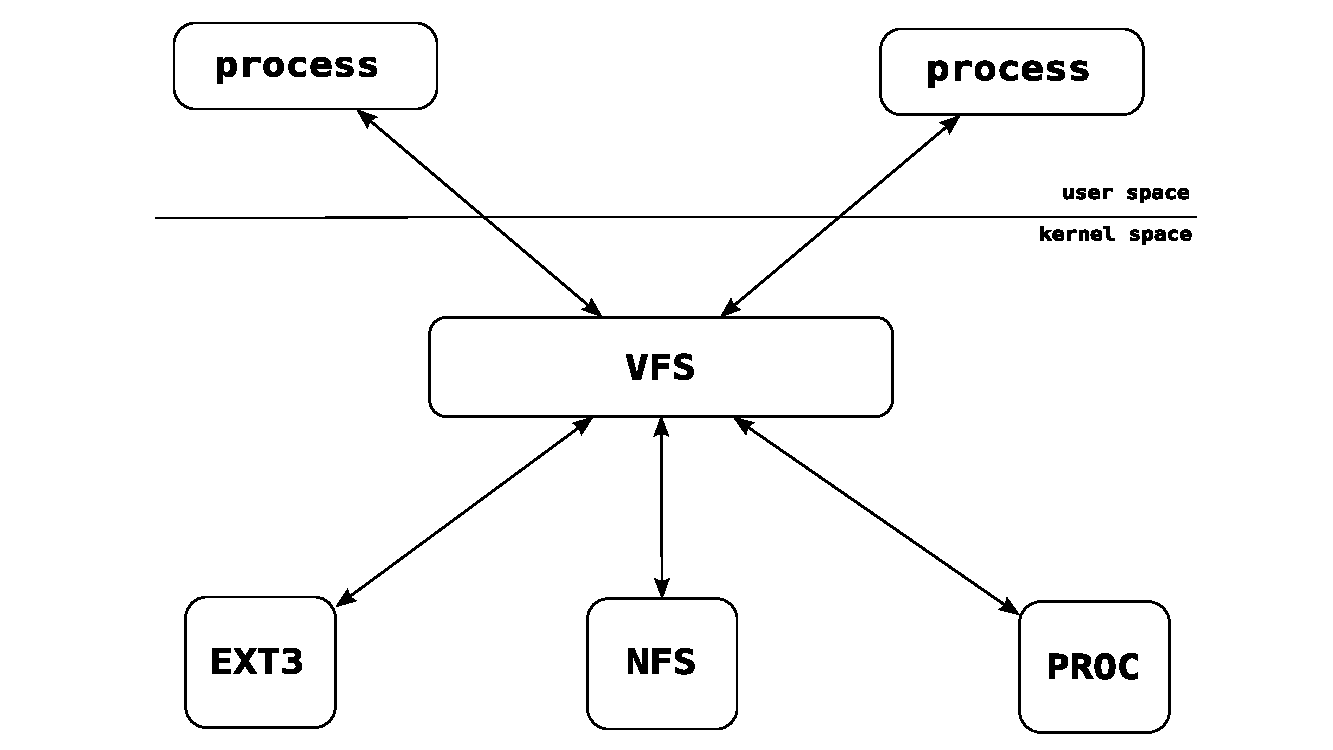
\includegraphics{vfs_role.pdf}
}

%-------------------------------------------------
\foilhead[-2cm]{VFS Objects}
\begin{itemize}
\item VFS object = data + table of operations
\item operations filled by filesystem
\end{itemize}

%-------------------------------------------------
\foilhead[-2cm]{Dentry Object}
\begin{itemize}
\item dentry -- directory entry
\item dentry object has no corresponding image on disk
\item used for pathname lookup
\item pathname lookup common for all filesystems
\item created for each path component
\item dentry has pointer to inode object
\end{itemize}

%-------------------------------------------------
\foilhead[-2cm]{Dentry Object}
\begin{itemize}
\item dentry without inode -- negative dentry (pathname lookup speed--up)
\item dentry objects are connected into the dentry tree
\item dentry cache + dentry hash table
\item dentry cache protected by \texttt{dcache\_lock}
\item dentry\_operations
\end{itemize}

%-------------------------------------------------
\foilhead[-2cm]{Dentries Created for Filename Path}
\fbox{
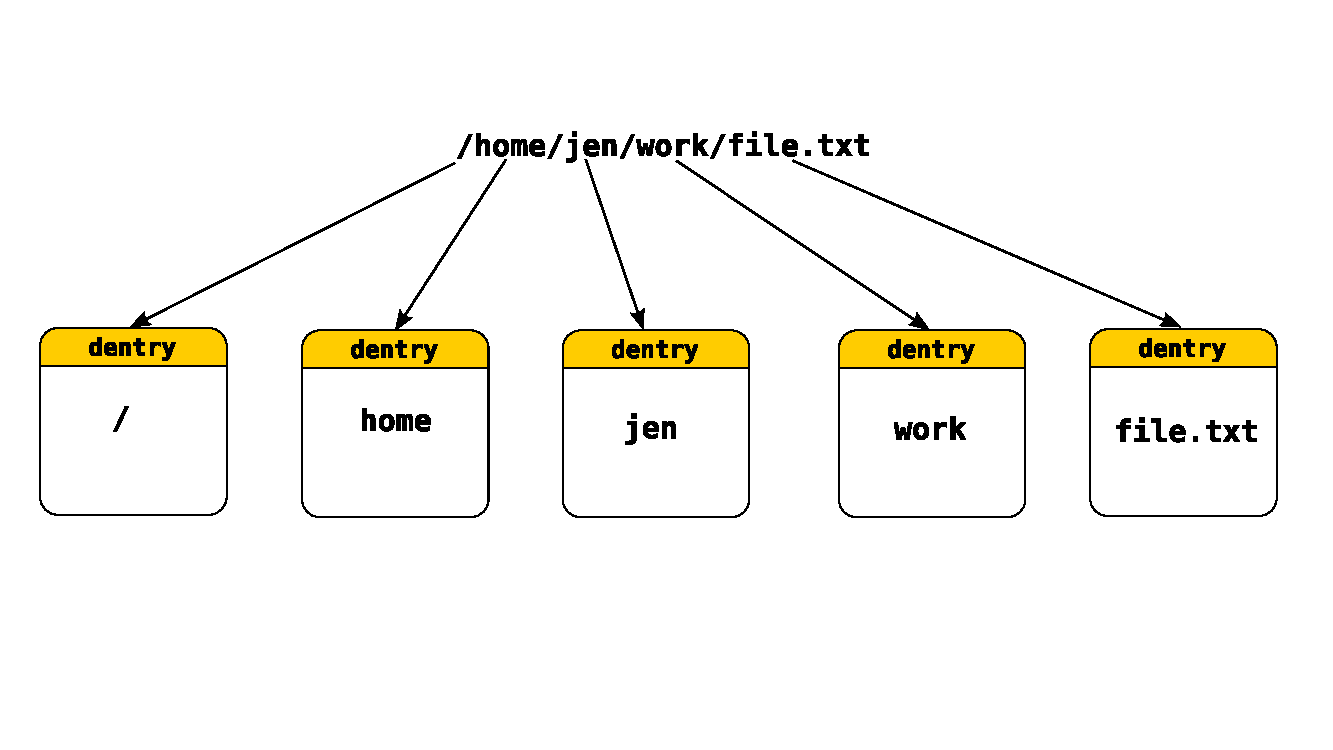
\includegraphics{dentry.pdf}
}

%-------------------------------------------------
\foilhead[-2cm]{Dentry Tree}
\fbox{
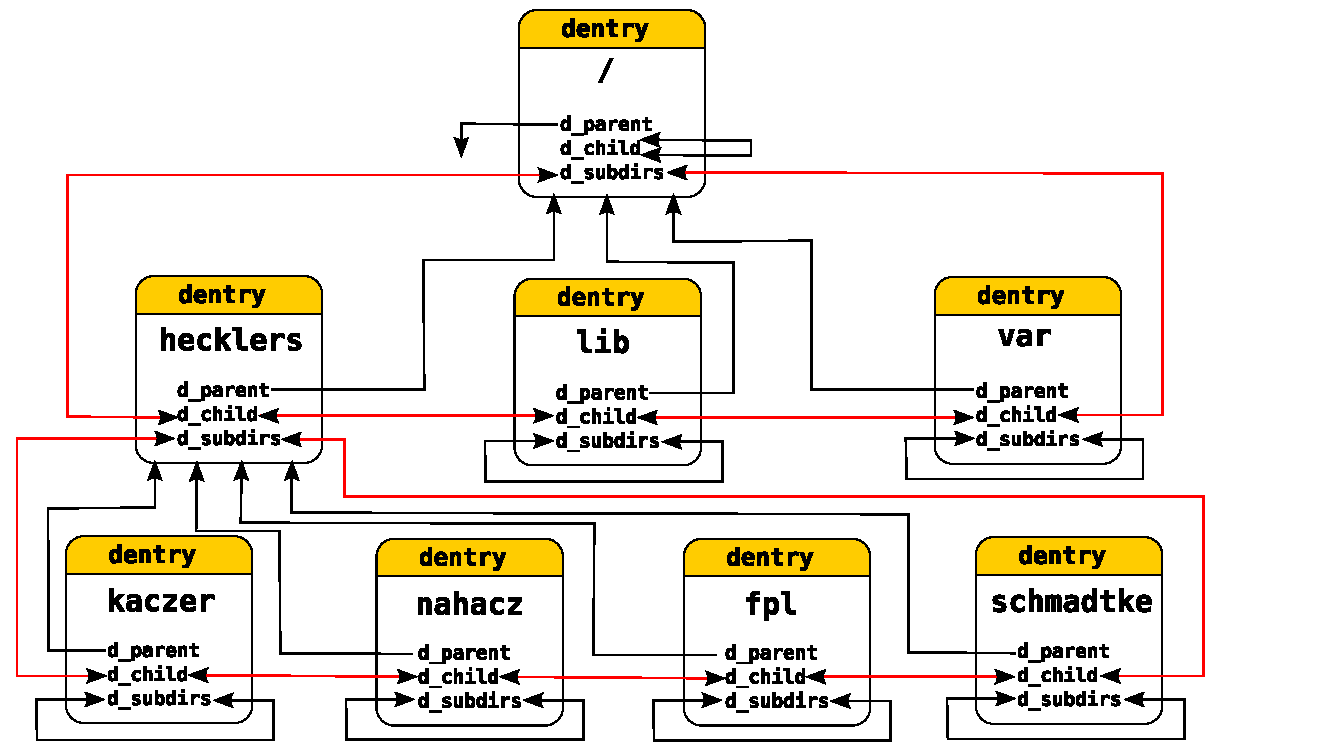
\includegraphics{dentry_tree.pdf}
}

%-------------------------------------------------
\foilhead[-2cm]{Inode Object}
\begin{itemize}
\item VFS inode vs. disk inode
\item duplicates some of the data in the disk inode
\item inode cache + inode hash table
\item inode does not contain name
\item list of dentry objects
\item inode\_operations
\item file\_operations
\end{itemize}

%-------------------------------------------------
\foilhead[-2cm]{Inode Object}
\begin{itemize}
\item contains address\_space object
\item buffer page cache
\item radix tree of inode pages (data)
\item address\_space operations
\end{itemize}

%-------------------------------------------------
\foilhead[-2cm]{File Object}
\begin{itemize}
\item created for each open call
\item contains file offset
\item contains pointer to dentry object
\item file\_operations
\item operations can be changed in the open operation (special files)
\end{itemize}

%-------------------------------------------------
\foilhead[-2cm]{VFS Objects Connections}
\fbox{
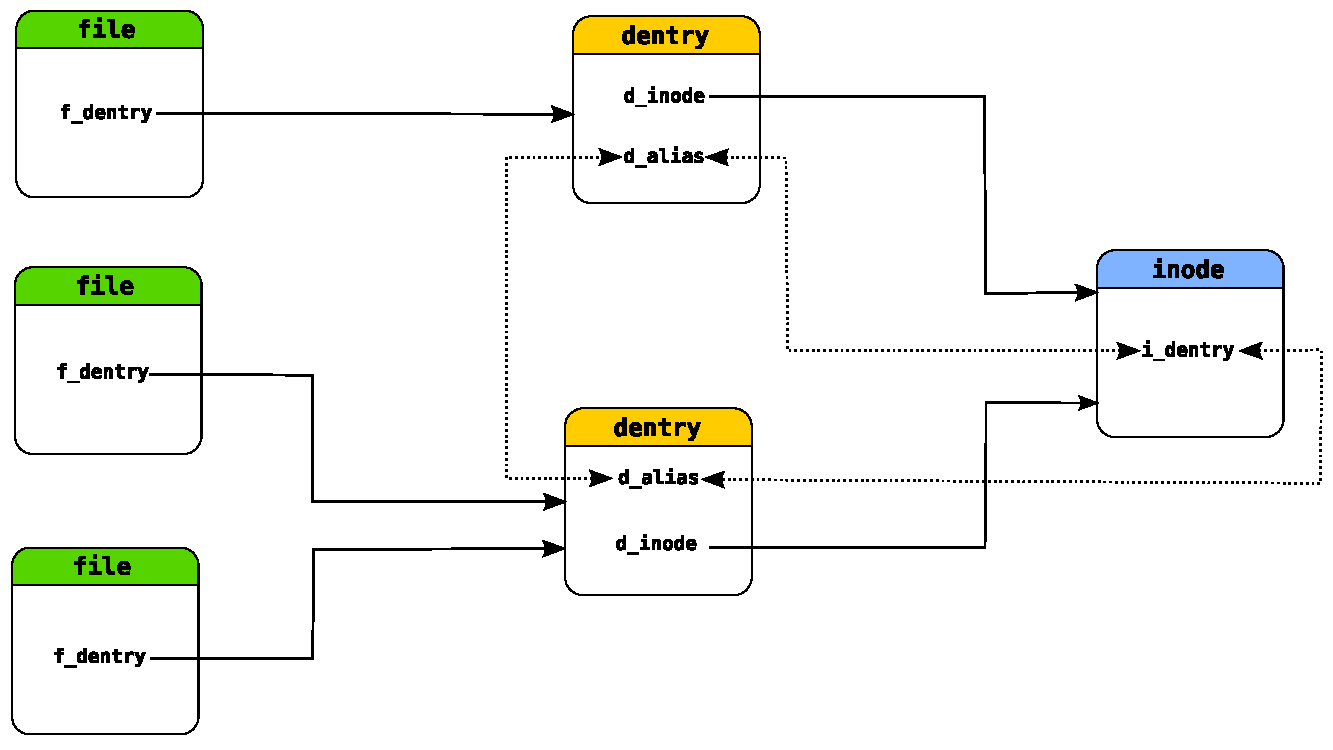
\includegraphics{vfs_objs_conn.pdf}
}

%-------------------------------------------------
\foilhead[-2cm]{File\_system\_type Object}
\begin{itemize}
\item thanks to this structure kernel knows that driver for filesystem is
available
\item contains filesystem name -- ext2, reiserfs
\item contains get\_sb operation
\item filled by filesystem
\item register\_filesystem
\item list of all file\_system\_type objects
\end{itemize}

%-------------------------------------------------
\foilhead[-2cm]{Superblock Object}
\begin{itemize}
\item dentry root object for filesystem
\item operations how to load and store data from and to filesystem
\item read\_inode, write\_inode
\item list of inodes
\item list of files
\end{itemize}

%-------------------------------------------------
\foilhead[-2cm]{Vfsmount Object}
\begin{itemize}
\item created for each mount point
\item Linux allows to stack multiple mounts on a single mount point
\item d\_mounted flag in dentry         
\end{itemize}

%-------------------------------------------------
\foilhead[-2cm]{Pathname Lookup}
\begin{itemize}
\item nameidata structure -- vfs\_mount and dentry
\item finds dentry (inode) for pathname         
\item d\_path reverse way 
\end{itemize}

%-------------------------------------------------
\foilhead[-2cm]{FiST: Stackable Filesystem}
\rightheader{FiST: Stackable Filesystem}
\begin{itemize}
\item File System Translator, Erez Zadok
\item supports Linux, FreeBSD, Solaris
\item code generator fistgen
\item ecryptfs -- vanilla kernel, based on cryptfs 
\item unionfs -- mm tree
\item uses Linux ability to mount one filesystem over other
\end{itemize}

%-------------------------------------------------
\foilhead[-2cm]{FiST: Stackable Filesystem}
\fbox{
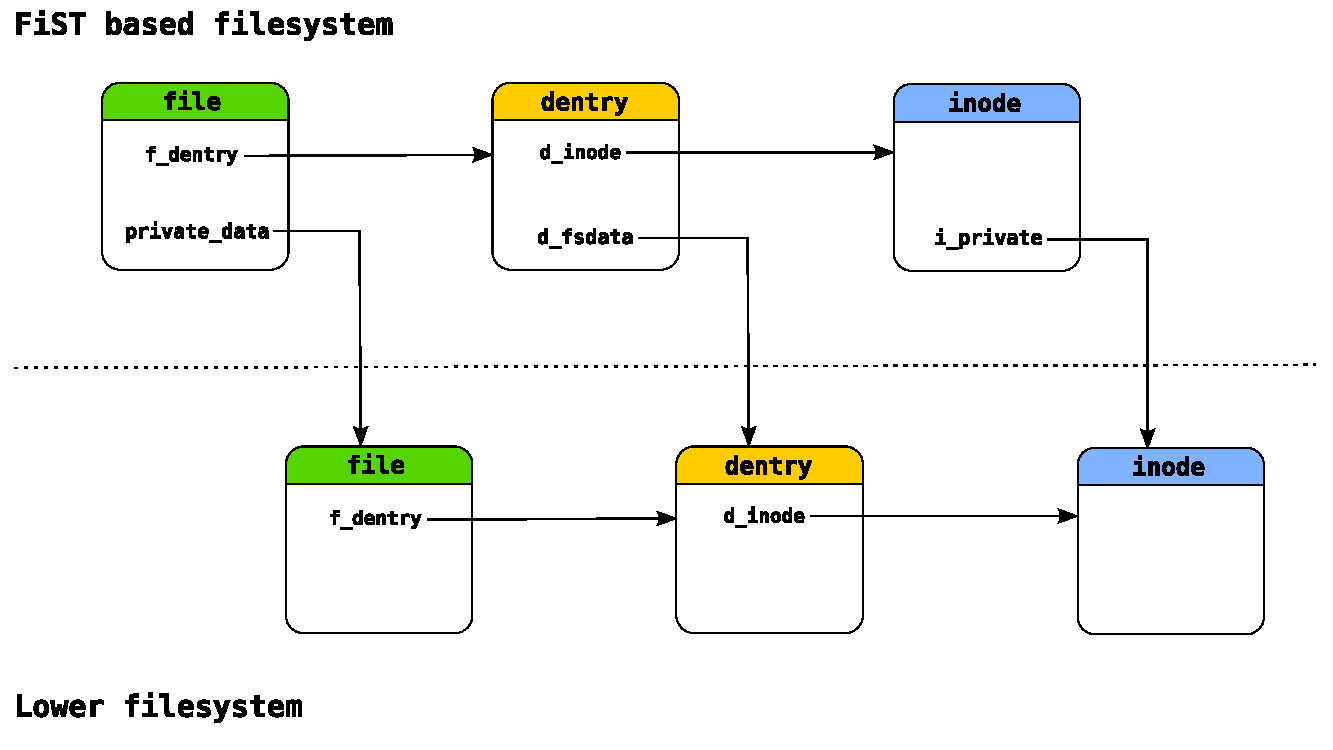
\includegraphics{fist.pdf}
}

%-------------------------------------------------
\foilhead[-2cm]{Linux Security Module}
\rightheader{Linux Security Module}
\begin{itemize}
\item first SELinux by NSA
\item set of security hooks to control operations on kernel objects 
\item security\_operations
\item only one security module registered directly to LSM -- master
\end{itemize}

%-------------------------------------------------
\foilhead[-2cm]{Dazuko: Access Control}
\rightheader{Dazuko: Access Control}
\begin{itemize}
\item founded by Avira GmbH (H+BDEV Datatechnik GmbH)
\item maintainer -- John Ogness
\item kernel module + user space library
\item mainly used for on-access scanning
\item Avira, AVG, NOD32, Avast!, Clam, F-Secure, AntiExploit
\item supports Linux and FreeBSD
\item system call table hooking, LSM, DazukoFS
\end{itemize}

%-------------------------------------------------
\foilhead[-2cm]{Redirecting FileSystem}
\rightheader{Redirecting Filesystem}

\begin{itemize}
\item allows to redirect file system calls in the VFS layer
\item is implemented as an out-of-kernel module for Linux 2.6
\item is able to register, unregister and manage one or more filters
\item allows filter to set its callback functions on-the-fly
\item allows filter to include and exclude its paths on-the-fly
\item allows filter to forward data from pre to post callback function
\item allows filter to attach its private data to VFS objects
\end{itemize}

%-------------------------------------------------
\foilhead[-2cm]{}
\begin{itemize}
\item allows filter to do subcalls for selected file system calls
\item calls pre and post callback function of filters in fixed order specified
by their priorities (call chain)
\item reacts on return value from filter and it is able to interrupt filters
call chain
\item redirects only operations selected by one or more filters, all other
operations go directly to the file system with no time overhead
\item modifies only VFS objects which belong to paths selected by one or more
filters
\end{itemize}

%-------------------------------------------------
\foilhead[-2cm]{Role}
\fbox{
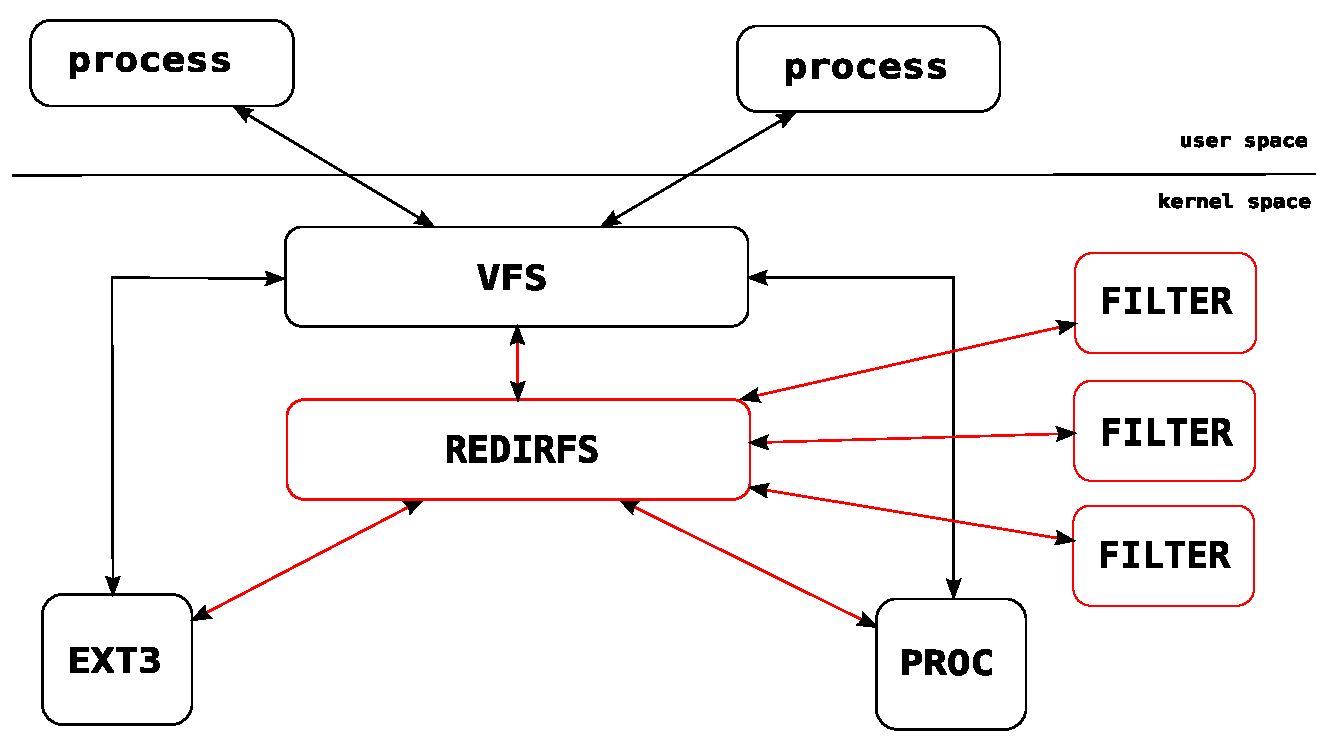
\includegraphics{rfs_role.pdf}
}

%-------------------------------------------------
\foilhead[-2cm]{Objects}
\begin{itemize}
\item for each VFS file, dentry, inode object is created corresponding RedirFS
rfile, rdentry, rinode object
\item RedirFS objects exists along with the corresponding VFS objects
\item rfile, rdentry and rinode objects are used as a connection with VFS
\item rdentry is created under d\_lock, rinode under i\_lock
\item rfile creation does not need locking
\end{itemize}

%-------------------------------------------------
\foilhead[-2cm]{Objects Connections}
\fbox{
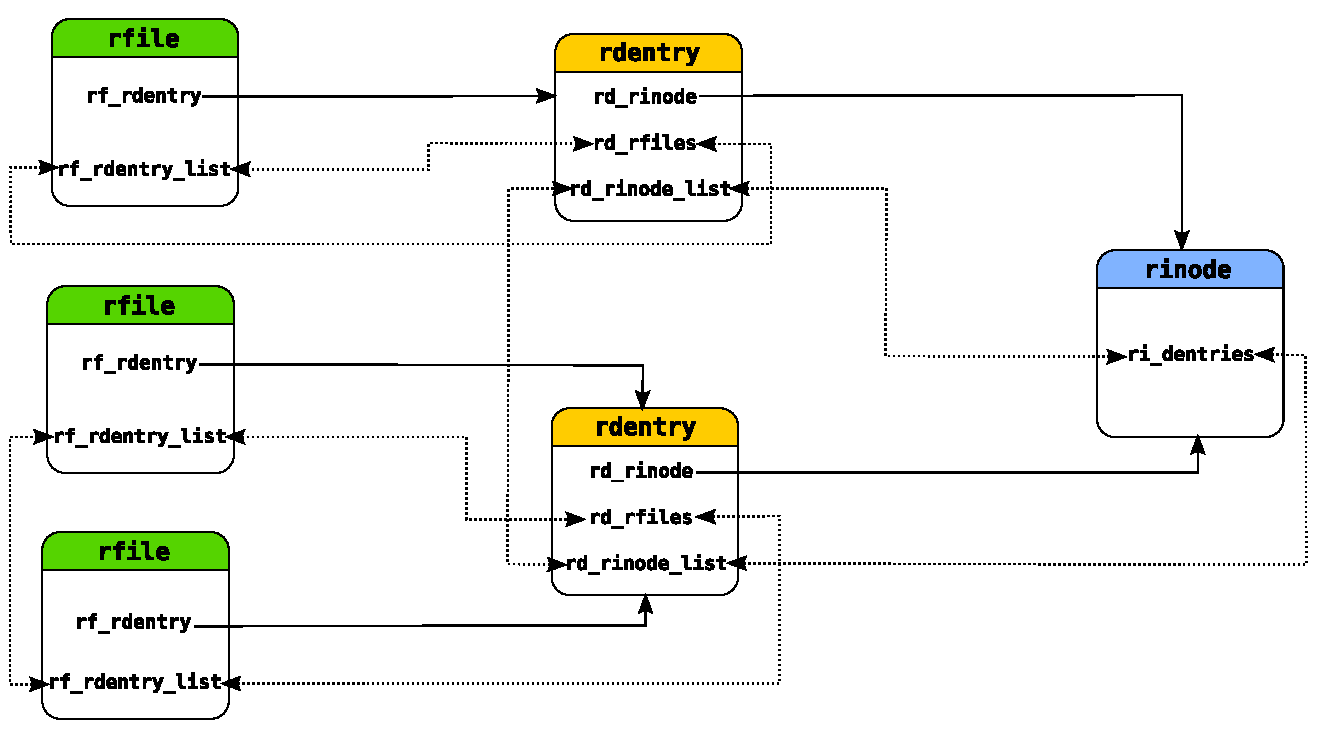
\includegraphics{rfs_vfs_objs_conn.pdf}
}

%-------------------------------------------------
\foilhead[-2cm]{VFS Object Operation Replacement}
\begin{itemize}
\item RedirFS is based on replacing of VFS objects operations
\item RedirFS is using the fact that pointer assignment in Linux kernel is
atomic
\item RedirFS creates new operations for each VFS object
\item new operations for VFS objects are embedded in RedirFS objects
\end{itemize}

%-------------------------------------------------
\foilhead[-2cm]{VFS Object Operation Replacement}
\begin{itemize}
\item replacement
\begin{enumerate}
\item alloc new operations
\item copy old operations
\item set new operations selected by filters callbacks
\item replace VFS object operations
\end{enumerate}
\end{itemize}

%-------------------------------------------------
\foilhead[-2cm]{VFS Object Operations Replacement}
\begin{itemize}
\item operation stays the same as original until one or more filters set
callback function for it
\item RedirFS needs to keep track of created and deleted VFS objects so it can
replace operations for newly created objects and on the other hand restore
operations when the VFS objects are deleted.
\end{itemize}

%-------------------------------------------------
\foilhead[-2cm]{VFS Object Operations Replacement}
\begin{itemize}
\item file\_operations -- open, release -- all, readdir -- dir
\item dentry\_operations -- d\_iput, d\_release -- all
\item inode\_operations -- mkdir, create, link, symlink, mknod -- dir, lookup --
all
\end{itemize}

%-------------------------------------------------
\foilhead[-2cm]{RedirFS and VFS connections}
\begin{itemize}
\item RedirFS =$>$ VFS: RedirFS object has pointer to VFS object
\item VFS =$>$ RedirFS: pointer of VFS object operations points to operations
stored within RedirFS object (container\_of macro)
\item Problem: VFS layer calls RedirFS operation but right before the
RedirFS object is obtained, it is deleted
\item Solution: RCU protected pointers to operations and fixed operations
(inode -- lookup, d\_iput -- dentry, open -- file)
\end{itemize}

%-------------------------------------------------
\foilhead[-2cm]{RedirFS Connection with VFS}
\fbox{
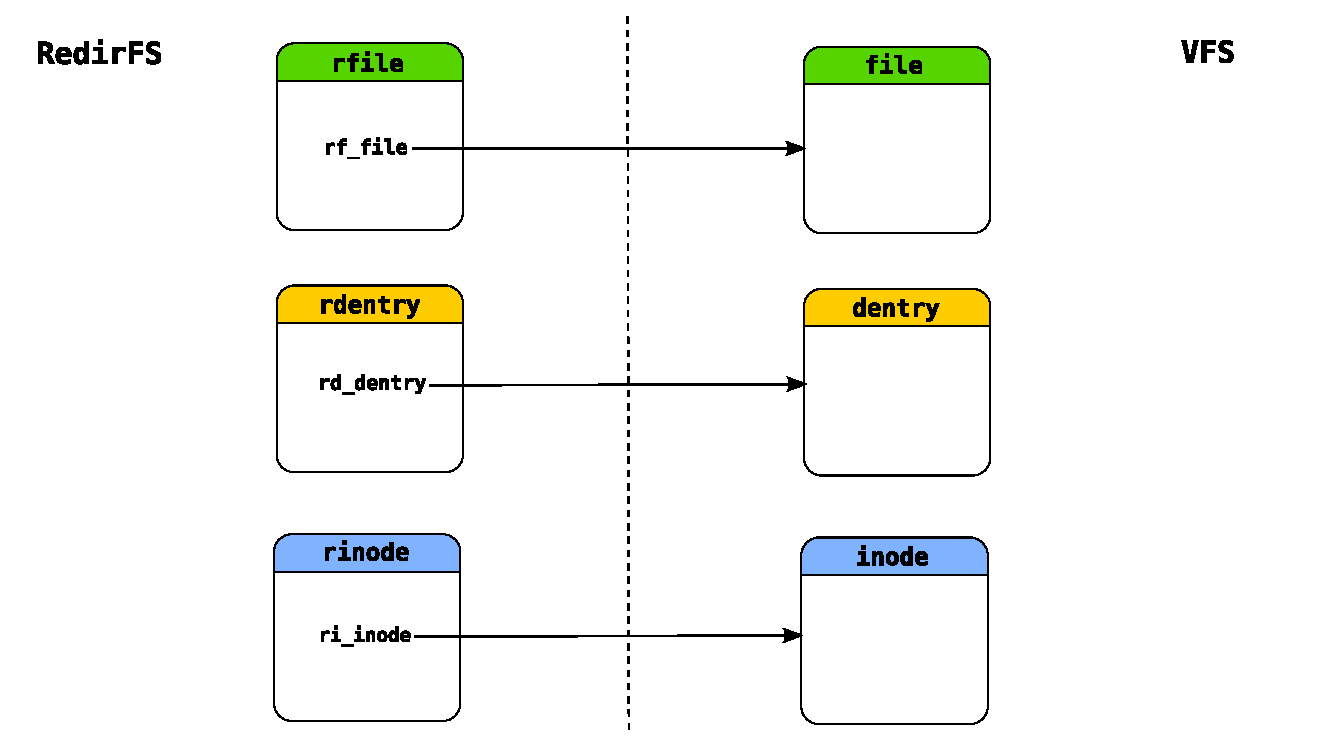
\includegraphics{rfs_vfs_conn.pdf}
}

%-------------------------------------------------
\foilhead[-2cm]{VFS Connection with RedirFS}
\fbox{
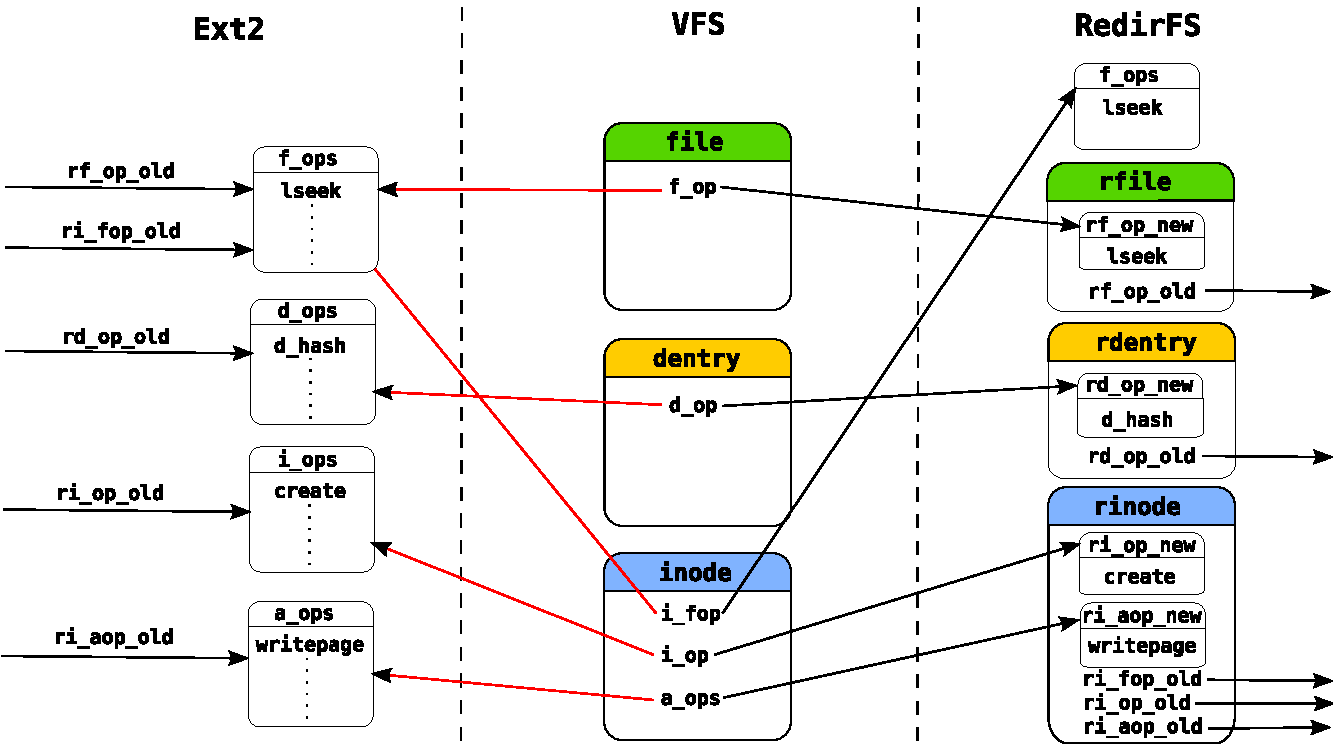
\includegraphics{vfs_rfs_conn.pdf}
}

%-------------------------------------------------
\foilhead[-2cm]{Walking Through the Dentry Cache}
\begin{itemize}
\item uses exported \texttt{dcache\_lock} and directory i\_mutex
\item dentry objects are connected into tree
\item dentry object has pointer to inode (negative dentry!)
\item replacing, restoring and setting VFS objects operations
\end{itemize}

\begin{lstlisting}[frame=trbl]{}
int rfs_walk_dcache(struct dentry *root, int flags,
		    int (*dcb)(struct dentry *dentry, void *dentry_data),
		    void *dcb_data,
		    int (*mcb)(struct dentry *dentry, void *dentry_data),
		    void *mcb_data)
\end{lstlisting}

%-------------------------------------------------
\foilhead[-2cm]{Filter}
\begin{itemize}
\item Filter in the RedirFS is represented by the filter structure. Each filter has a
name, a unique priority number, a set of pre and post callback operations and a
set of paths
\end{itemize}

%-------------------------------------------------
\foilhead[-2cm]{Filters Call Chain}
\begin{itemize}
\item each RedirFS object contains so called filters call chain
\item filters call chain is a list of filters which are interested in one or
more operations of the VFS object sorted according to their priorities
\item this list tells RedirFS which Filters have to be called before (pre
callbacks) and after (post-callbacks) the original operation
\end{itemize}

%-------------------------------------------------
\foilhead[-2cm]{Filters Call Chain}
\begin{itemize}
\item filter can finish or stop the proceeding operation in its pre callback
function
\item post callback functions are called for each filter for which its pre
callback function was called
\end{itemize}

%-------------------------------------------------
\foilhead[-2cm]{Subcalls}
\begin{itemize}
\item subcalls are RedirFS functions for selected VFS operations
\item subcall calls only filters which are in the filter call chain past the
filter which called the subcall
\item subcalls allow filter to call the same VFS operation with its own or
modified arguments
\item subcalls also allow filter to call different operations
\end{itemize}

%-------------------------------------------------
\foilhead[-2cm]{Private Data}
\begin{itemize}
\item filters are allowed to attach their private data to file,
inode, dentry
\item synchronization needed
\item private data for filters are kept in a list in the RedirFS object
corresponding to the VFS object
\item filter can attach private data per operation in the pre callback function
\item filter has to detach them in the post callback function
\end{itemize}

%-------------------------------------------------
\foilhead[-2cm]{Path Management}
\begin{itemize}
\item paths selected by filters are in the RedirFS represented by the
\texttt{rpath} structure
\item filters can include or exclude directory subtrees or even single path
(file or directory)
\item rpath objects are connected in trees and the root of each tree
is stored in the global \texttt{path\_list} list
\end{itemize}

%-------------------------------------------------
\foilhead[-2cm]{Path Management}
\begin{itemize}
\item rpath has lists of filters call chains -- \texttt{p\_inchain, p\_exchain,
p\_inchain\_local, p\_exchain\_local}
\item rpath has operations for VFS objects belonging to it
\item filter can not set fixed paths
\end{itemize}

%-------------------------------------------------
\foilhead[-2cm]{Path Tree}
\fbox{
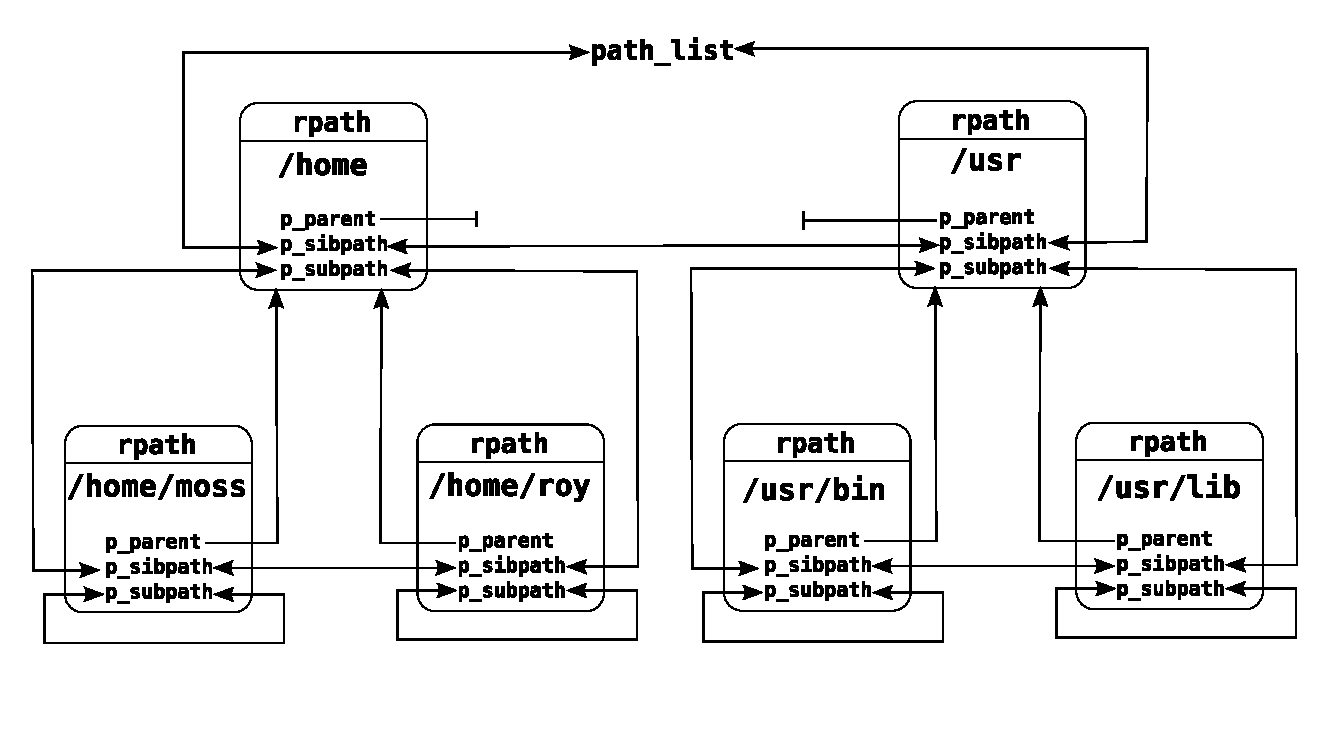
\includegraphics{rfs_paths.pdf}
}

%-------------------------------------------------
\foilhead[-2cm]{Walking Through Paths}
\begin{itemize}
\item  rpath borders for \texttt{rfs\_walk\_dcache} are stored in rdentry --
\texttt{rd\_root}
\end{itemize}

\begin{lstlisting}[frame=trbl]{}
int rfs_path_walk(struct rpath *path, int walkcb(struct rpath*, void*),
                  void *datacb);
\end{lstlisting}

%-------------------------------------------------
\foilhead[-2cm]{Sysfs Interface}
\begin{itemize}
\item RedirFS creates same basic attributes for each filter in the sysfs
file system. For each filter is created a directory /sys/fs/redirfs/$<$filter
name$>$ with following files (attributes)
\item active -- activated or deactivated filter 
\item paths -- included and excluded paths, path can be set via this file
\item control -- flag if filter is accepting setting via the sysfs
\item priority -- filter's priority
\end{itemize}

%-------------------------------------------------
\foilhead[-2cm]{Objects Connections}
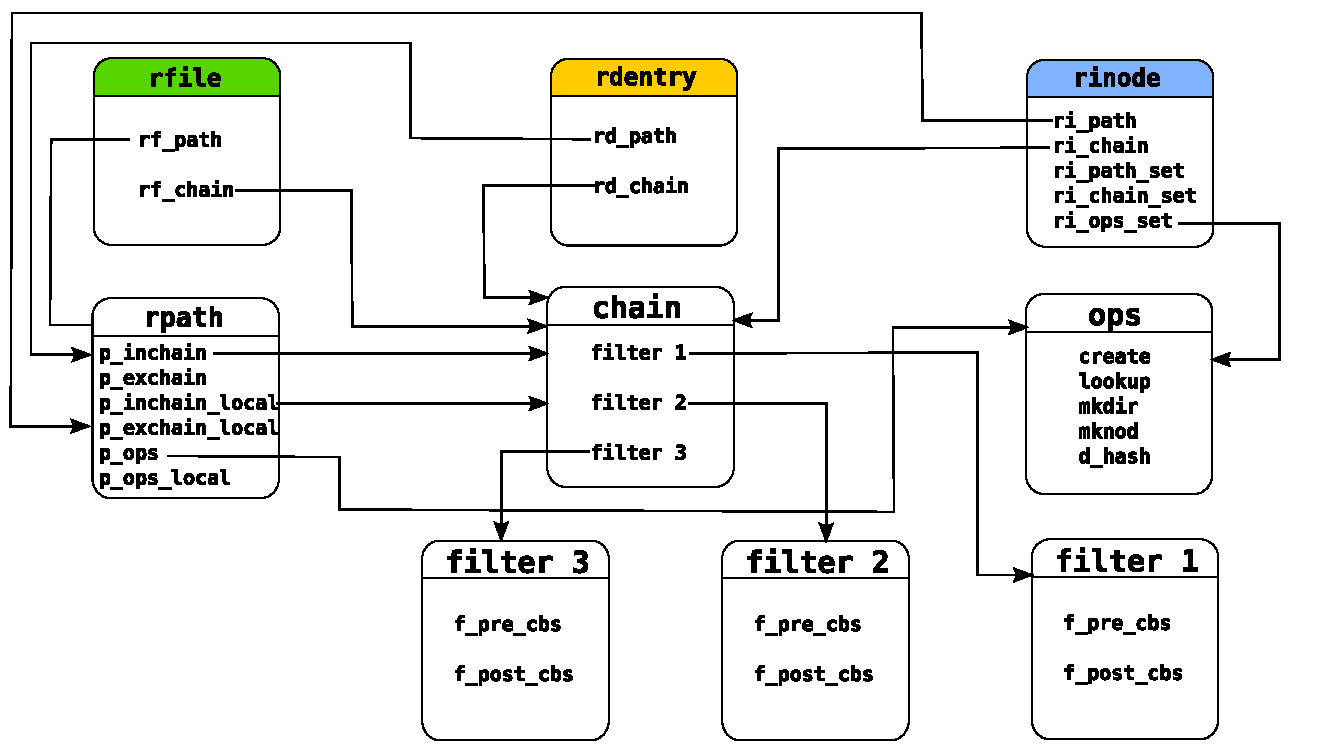
\includegraphics{rfs_objs_conn.pdf}

%-------------------------------------------------
\foilhead[-2cm]{Filters}
\rightheader{Filters}

\begin{itemize}
\item filter is a linux kernel module (LKM) using the RedirFS framework
\item filter can add some useful functionality to existing filesystems like
transparent compression, transparent encryption, merging contents of several
directories into the one, allowing writing to a read-only media and other
\item filter has a unique number called priority which defines its order in the
filter call chain
\end{itemize}

%-------------------------------------------------
\foilhead[-2cm]{Filters}
\begin{itemize}
\item filter defines a set of pre and post callback functions for selected
filesystem calls
\item filter defines paths over which its callback functions will be called
\item filter can include or exclude paths as a subtrees or as a single paths
\end{itemize}

%-------------------------------------------------
\foilhead[-2cm]{Registration \& Unregistration}
\begin{itemize}
\item filter registered to RedirFS is identified by a handle
\item registration requires properly filled \texttt{rfs\_filter\_info}
\end{itemize}

\begin{lstlisting}[frame=trbl]{}
rfs_filter filter;

struct rfs_filter_info {
        char *name;
        int priority;
        int active;
        int (*ctl_cb)(struct rfs_ctl *ctl);
};

int rfs_register_filter(rfs_filter *flt, struct rfs_filter_info *filter_info);

int rfs_unregister_filter(rfs_filter filter);
\end{lstlisting}

%-------------------------------------------------
\foilhead[-2cm]{Activation \& Deactivation}
\begin{itemize}
\item filter can be active or inactive
\item RedirFS calls only active filters
\item filter's state can be set during registration
\item filter's state can be changed anytime after registration
\end{itemize}
\begin{lstlisting}[frame=trbl]{}
int rfs_activate_filter(rfs_filter filter);
int rfs_deactivate_filter(rfs_filter filter);
\end{lstlisting}

%-------------------------------------------------
\foilhead[-2cm]{Operations Settings}
\begin{itemize}
\item filter can register pre and post callback functions for selected
filesystem calls
\item each operation is described by the \texttt{rfs\_op\_info} structure
\end{itemize}

\begin{lstlisting}[frame=trbl]{}
struct rfs_op_info {
        enum rfs_op_id op_id;
        enum rfs_retv (*pre_cb)(rfs_context, struct rfs_args *);
        enum rfs_retv (*post_cb)(rfs_context, struct rfs_args *);
};
static struct rfs_op_info op_info[] = {
        {RFS_DIR_IOP_PERMISSION, NULL, dummyflt_permission},
        {RFS_REG_FOP_OPEN, dummyflt_open, NULL},
        {RFS_OP_END, NULL, NULL}
};
int rfs_set_operations(rfs_filter filter, struct rfs_op_info *op_info);
\end{lstlisting}

%-------------------------------------------------
\foilhead[-2cm]{Filter's Callback Functions}

\begin{itemize}
\item all pre and post callback functions have the same interface
\item filter can stop filters call chain
\item filter can modify or replace original operation arguments
\end{itemize}

\begin{lstlisting}[frame=trbl]{}
enum rfs_retv cb(rfs_context cont, struct rfs_args*rargs);

struct rfs_args {
        union rfs_op_args args;
        union rfs_op_retv retv;
        struct rfs_op_type type;
};
\end{lstlisting}

%-------------------------------------------------
\foilhead[-2cm]{Paths Settings}
\begin{itemize}
\item include or exclude -- \texttt{\small{RFS\_PATH\_INCLUDE,
RFS\_PATH\_EXCLUDE}}
\item subtree or single path -- \texttt{\small{RFS\_PATH\_SUBTREE,
RFS\_PATH\_SINGLE}}
\item filter can not set fixed paths
\end{itemize}

\begin{lstlisting}[frame=trbl]{}
struct rfs_path_info {
        char *path;
        int flags;
}

int rfs_set_path(rfs_filter filter, struct rfs_path_info *path_info);
\end{lstlisting}

%-------------------------------------------------
\foilhead[-2cm]{Control Callback Function}
\begin{itemize}
\item request for new settings entered through the sysfs interface
\item filter can decide if it will follow new settings or just ignore it
\item only settings common for all filters
\item \texttt{\small{RFS\_CTL\_ACTIVATE, RFS\_CTL\_DEACTIVATE,
RFS\_CTL\_SETPATH}}
\end{itemize}

\begin{lstlisting}[frame=trbl]{}
struct rfs_ctl {
        enum rfs_ctl_id id;
        union rfs_ctl_data data;
};
\end{lstlisting}


%-------------------------------------------------
\foilhead[-2cm]{Sysfs Interface}
\begin{itemize}
\item for each filter has a directory \texttt{\small{/sys/fs/redirfs/<filter name>}}
\item sysfs attributes -- active, control, priority, paths
\end{itemize}

\begin{lstlisting}[frame=trbl]{}
int rfs_register_attribute(rfs_filter flt, struct rfs_flt_attribute *attr);
int rfs_unregister_attribute(rfs_filter flt, struct rfs_flt_attribute *attr);

struct rfs_flt_attribute {
	struct attribute attr;
	ssize_t (*show)(rfs_filter flt, struct rfs_flt_attribute *attr,
	                char *buf);
	ssize_t (*store)(rfs_filter flt, struct rfs_flt_attribute *attr,
	                 const char *buf, size_t size);
	void *data;
};
#define rfs_flt_attr(__name, __mode, __show, __store, __data)
\end{lstlisting}

%-------------------------------------------------
\foilhead[-2cm]{Private Data for VFS objects}
\begin{itemize}
\item filter can attach, detach and get its private data for file, dentry and inode
\end{itemize}

\begin{lstlisting}[frame=trbl]{}
int rfs_attach_data_inode(rfs_filter filter, struct inode *inode,
                          struct rfs_priv_data *data,
			  struct rfs_priv_data **exist);
int rfs_detach_data_inode(rfs_filter filter, struct inode *inode,
                          struct rfs_priv_data **data);
int rfs_get_data_inode(rfs_filter filter, struct inode *inode,
                       struct rfs_priv_data **data);

int rfs_init_data(struct rfs_priv_data *data, rfs_filter filter,
                  void (*cb)(struct rfs_priv_data *));

void rfs_put_data(struct rfs_priv_data *data);
struct rfs_priv_data *rfs_get_data(struct rfs_priv_data *data);
\end{lstlisting}

\foilhead[-2cm]{Private Data for Operation Context}
\begin{itemize}
\item filter can attach its private data per operation and pass it from pre to
post callback function
\item filter has to detach its private data in the post callback function
\end{itemize}

\begin{lstlisting}[frame=trbl]{}
int rfs_init_data_cont(struct rfs_cont_data *data, rfs_filter filter);
int rfs_attach_data_cont(rfs_filter filter, rfs_context *context,
                         struct rfs_cont_data *data);
int rfs_detach_data_cont(rfs_filter filter, rfs_context context,
                         struct rfs_cont_data **data);
\end{lstlisting}

%-------------------------------------------------
\foilhead[-2cm]{Subcalls}
\begin{itemize}
\item RedirFS functions for selected VFS operations
\item subcall calls only filters which are in the filter call chain past the
filter which called the subcall
\item \texttt{\small{<type> rfs\_<name>\_subcall(rfs\_filter flt, union
rfs\_op\_args *args);}}
\end{itemize}

\begin{lstlisting}[frame=trbl]{}
ssize_t rfs_read_subcall(rfs_filter flt, union rfs_op_args *args);
ssize_t rfs_aio_read_subcall(rfs_filter flt, union rfs_op_args *args);
int rfs_readpage_subcall(rfs_filter flt, union rfs_op_args *args);
ssize_t rfs_write_subcall(rfs_filter flt, union rfs_op_args *args);
\end{lstlisting}

%-------------------------------------------------
\foilhead[-2cm]{}
\rightheader{Questions}
\vspace{1cm}
\begin{center}
\Huge{Thanks for your attention}
\end{center}
\vspace{2cm}
\begin{center}
\Huge{Questions?}
\end{center}


%-------------------------------------------------
\foilhead[-2cm]{References}
\rightheader{References}

\begin{itemize}
\item Bovet, P. B., Cesati, M.: Understanding the Linux Kernel. 3rd Edition, U.S.A., O'Reilly 2005
\item Love, R.: Linux Kernel Development. 2nd Edition, Indianapolis, Indiana, Novel Press 2005
\item Alessandro Rubini, Jonathan Corbet: Linux Device Drivers, 2nd Edition, U.S.A., O'Reilly 2001
\item www.filesystems.org, www.dazuko.org
\item http://www.nsa.gov/selinux/papers/module/t1.html
\end{itemize}

\end{document}

